%%%%%%%%%%%%%%%%%%%%%%%%%%%%%%%%%%%%%%%%%%%%%%%%%%%%%%%%%%%%%%%%%%%%%%%%%%%%%%%
% Chapter 'Adsorption - Ethanol - activated carbon ATO'
%%%%%%%%%%%%%%%%%%%%%%%%%%%%%%%%%%%%%%%%%%%%%%%%%%%%%%%%%%%%%%%%%%%%%%%%%%%%%%%
\subsection{Activated carbon ATO}
%
%%%%%%%%%%%%%%%%%%%%%%%%%%%%%%%%%%%%%%%%%%%%%%%%%%%%%%%%%%%%%%%%%%%%%%%%%%%%%%%
%%%%%%%%%%%%%%%%%%%%%%%%%%%%%%%%%%%%%%%%%%%%%%%%%%%%%%%%%%%%%%%%%%%%%%%%%%%%%%%
\subsubsection{DubininAstakhov - ID 1}
%
\begin{tabular}[l]{|lp{11.5cm}|}
\hline
\addlinespace

\textbf{Sorbent:} & activated carbon \\
\textbf{Subtype:} & ATO \\
\textbf{Refrigerant:} & Ethanol \\
\textbf{Equation:} & DubininAstakhov \\
\textbf{ID:} & 1 \\
\textbf{Reference:} & Brancato, V.; Frazzica, A.; Sapienza, A.; Gordeeva, L.; Freni, A. (2015): Ethanol adsorption onto carbonaceous and composite adsorbents for adsorptive cooling system. In: Energy 84, S. 177–185. DOI: 10.1016/j.energy.2015.02.077. \\
\textbf{Comment:} & None \\

\addlinespace
\hline
\end{tabular}
\newline

\textbf{Properties of sorbent:}
\newline
%
\begin{longtable}[l]{lll}
\toprule
\addlinespace
\textbf{Property} & \textbf{Unit} & \textbf{Value} \\
\addlinespace
\midrule
\endhead
\bottomrule
\endfoot
\bottomrule
\endlastfoot
\addlinespace

Diameter of pore & \si{\milli\meter} & 0.00000118\\
Diameter of pellet & \si{\milli\meter} & 0.25-0.6\\
Surface area & \si{\square\meter\per\gram} & 1745\\
Pore volume & \si{\milli\cubic\meter\per\gram} & 0.64\\

\addlinespace\end{longtable}

\textbf{Equation and parameters:}
\newline
%
Loading $w$ in $\si{\kilogram\per\kilogram}$ is calculated depending on pressure $p$ in $\si{\pascal}$, temperature $T$ in $\si{\kelvin}$, and vapor pressure $p_\mathrm{sat}$ in $\si{\pascal}$ by:
%
\begin{equation*}
\begin{split}
w &=& \begin{cases} W \rho_\mathrm{sat}^{\mathrm{liq}} & \quad \text{if flag} \geq 0 \\ W & \quad \text{else} \end{cases} & \quad\text{, and} \\
W &=& W_0 \exp \left( - \left( \nicefrac{A}{E} \right) ^{n} \right) & \quad\text{, and} \\
A &=& R T \ln \left( \nicefrac{p_\mathrm{sat}}{p} \right) & \quad\text{.} \\
\end{split}
\end{equation*}
%
The parameters of the equation are:
%
\begin{longtable}[l]{lll|lll}
\toprule
\addlinespace
\textbf{Par.} & \textbf{Unit} & \textbf{Value} &	\textbf{Par.} & \textbf{Unit} & \textbf{Value} \\
\addlinespace
\midrule
\endhead

\bottomrule
\endfoot
\bottomrule
\endlastfoot
\addlinespace

flag & - & 1.000000000e+00 & $n$ & - & 1.700000000e+00 \\
$E$ & $\si{\joule\per\mole}$ & 1.120000000e+04 & $W_0$ & $\si{\cubic\meter\per\kilogram}$ & 6.100000000e-04 \\

\addlinespace\end{longtable}

\textbf{Validity:}
\newline
Equation is approximately valid for $1260.0 \si{\pascal} \leq p \leq 3540.0 \si{\pascal}$,  $303.097 \si{\kelvin} \leq T \leq 393.127 \si{\kelvin}$, and $0.04335 \si{\kilogram\per\kilogram} \leq w \leq 0.42683 \si{\kilogram\per\kilogram}$.
\newline

\textbf{Visualization:}
%
\begin{figure}[!htp]
{\noindent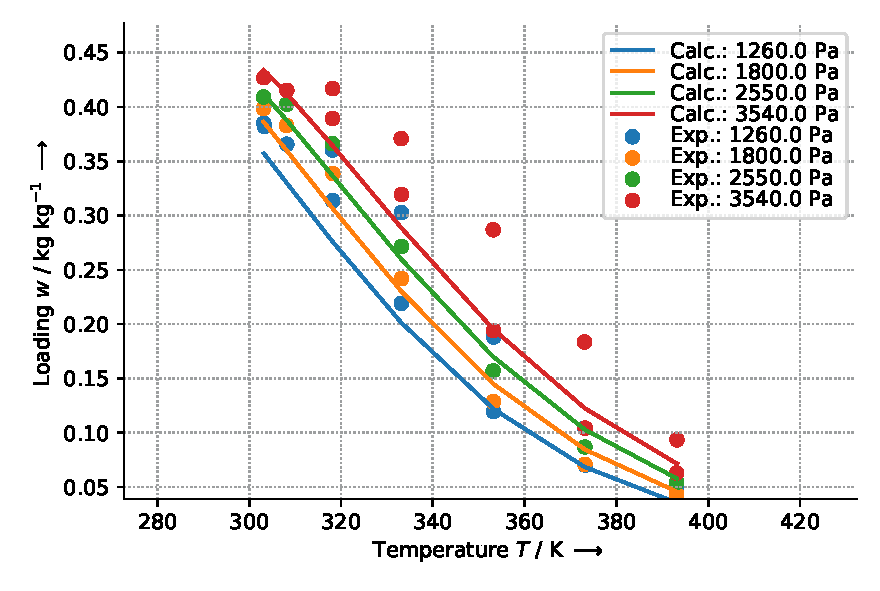
\includegraphics[height=10cm, keepaspectratio]{figs/ads/ads_Ethanol_activated_carbon_ATO_DubininAstakhov_1.pdf}}
\end{figure}
%

To generate the figure, the following refrigerant functions were selected:
\begin{itemize}
\item Vapor pressure: VaporPressure\_EoS1 - ID 1
\item Saturated liquid density: SaturatedLiquidDensity\_EoS1 - ID 1
\end{itemize}

The uncertainity of the experimental data is:
\begin{itemize}
\item Data source $\,\to\,$ Data was taken from figure
\item Pressure, absolute, in $\si{\pascal}$ $\,\to\,$ 420
\end{itemize}

The mean absolute percentage error (MAPE) between the experimental and calculated data results in 12.57\%.
\FloatBarrier
\newpage
%%%%%%%%%%%%%%%%%%%%%%%%%%%%%%%%%%%%%%%%%%%%%%%%%%%%%%%%%%%%%%%%%%%%%%%%%%%%%%%
